\documentclass{article}
\usepackage{graphicx}
\usepackage{float}
\usepackage{hyperref}
\usepackage[bottom]{footmisc}

\begin{document}
	
	\title{Of digestive biscuits, old leather, and smoked ham: making sense of the language of Scotch whisky}
	\author{Praveen Gowtham}
	\date{}
	\maketitle
	
	\section{Motivation}
	\paragraph{} Somewhere in the world -- even as we speak -- there is a group of friends sitting near a fireplace in a cozy house. It's autumn and its damp and starting to get a bit chilly outside. The friends are warm. There is soft talking and thoughtful pauses. There are glasses in their hands. Golden red elixir swooshes back and forth. One of them hold the glass up to the fire, sees light dancing through gold, swishes the glass and tilts. Fingers of liquid gold slide down the side of the glass. Now the glass goes up to the mouth: a slow slip. The mouth chews the liquid. Swallows. Inhales and exhales.
	
	Then the mouth speaks: "I think I'm getting some orange peel, maybe a little pepper in the finish."
	
	There is a small pause. 
	
	Then another voice: "I've got some red chilli and a bit of oak."
	
	The rest ponder these statements. Orange and shadow flickers over faces.
	
	\paragraph{} The question is: are these people agreeing? Are they saying similar things but using different descriptors? Or are they tasting very different things? Taste and smell are tricky to delineate. After a few simple common descriptors (sweet, spicy, etc.) one immediately finds oneself in the jungle of metaphor and simile. And Scotch single malt whisky can be a complex thing indeed. There are many (in some cases, rather strange) similies/metaphors used to describe Scotch. The goal of this work is to try and build a list of words used to describe the tastes and smell of Scotch and then to discover groups of such descriptors. The hope is that these groups give us general types of flavor/smell profiles present in the entire domain of Scotch whisky. This will also help us to understand a given Scotch's taste profile by its breakdown according to these groups.
	
	\section{Background}
	 
	 Scotch is a spirit made from fermenting the sugars of malted barley and distilling the product. The distilled liquid is then aged for years in barrels that once used to hold other products (sherry, wine, bourbon, etc.). There are many factors that affect the final flavor of a whisky. A master distiller toys with all of these with specific end tastes, smells, and textures in mind. Such factors include: type of fuel used in the kiln firing to dry barley after germination, shape/size of the stills and geometry of the condensers, the times and temperatures where distilled liquid is discarded or set aside, the types of casks/barrels used in aging and the time they spend in each. Then, of course, there is the terroir: the air, the surroundings, and water. The process is complex with many interconnected variables and this results in Scotch flavor profiles that are intricate and multilayered.
	 Expert tasters and distillers have developed a language to discuss these flavor profiles. Much of this language has trickled down to Scotch enthusiasts and probably even to our friends sitting in a house on a chilly autumn day.
	 \begin{figure}[H]
		\begin{center}
			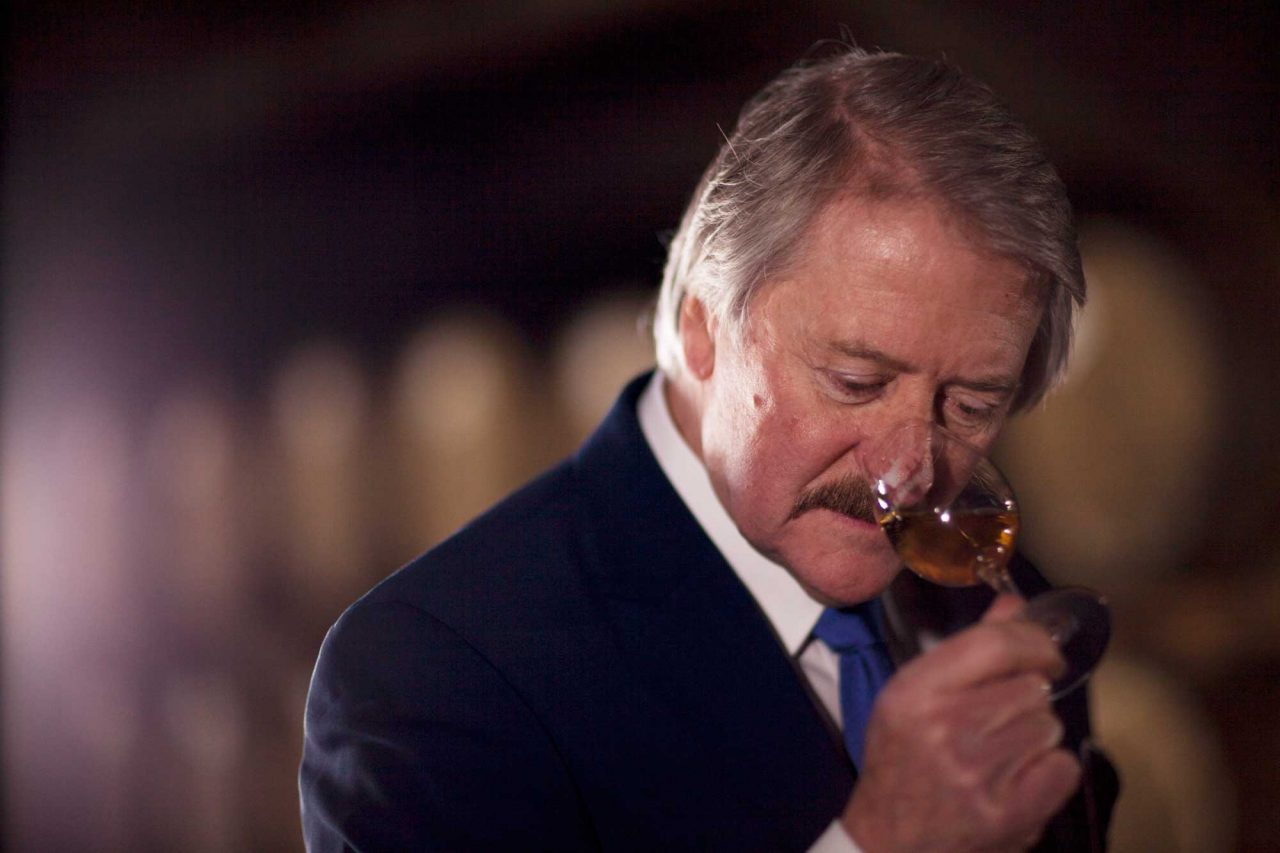
\includegraphics[totalheight=6cm]{figures/richpaterson_expert.jpg}
		\end{center}
		\caption{Master blender and expert taster Richard Paterson getting his honker in there.}
	\end{figure}
	 
	 \section{Data Wrangling}
	 \subsection{Data Sources}
	 \paragraph{}Master of Malt (MoM) is a pretty good repository for such flavor descriptions of Scotch whisky. The Chaps at MoM  are expert tasters that have quite possibly tasted nearly every Scotch whisky in existence. Their website is an encyclopedia of tasting notes on these scotches and contains a whole host of other information (price, age, ABV, type of casks used, etc.) as well. We scraped approximately 14,000 descriptions on single malt Scotches from MoM's website using scrapy. The start url for our scrapy spider is: \\ \href{https://www.masterofmalt.com/country-style/scotch/single-malt-whisky/}{https://www.masterofmalt.com/country-style/scotch/single-malt-whisky/} \\
	 
	 The atrributes scraped for each Scotch are listed below:
	 
	 \begin{table}[H]
	 	\begin{tabular}{|c|c|}
	 		\hline
	 		name &  The name of the scotch.\\
	 		\hline
	 		distillery &  Distillery that produced the scotch.\\
	 		\hline
	 		bottler &  Some scotches are aged/bottled by 3rd parties. \\
	 		\hline
	 		region & Whisky making region that the distillery belongs to. \\
	 		\hline
	 		age & Maturation time (in years).  \\
	 		\hline
	 		ABV & Alcohol by volume. \\
	 		\hline
	 		price & MoM is also a store. Price in USD.  \\
	 		\hline
	 		description & General notes about the Scotch.  \\
	 		\hline
	 		nose & Free text description of the scent of the Scotch.  \\
	 		\hline
	 		palate & Free text description of the taste of the whisky. \\
	 		\hline
	 		finish & Free text description of aftertastes.  \\
	 		\hline
	 		chill filter & Is the whisky chill filtered? \\
	 		\hline
	 		cask strength & Is the whisky bottled at cask strength? \\
	 		\hline
	 		maturation & Info about the type of cask(s) used to age the whisky. \\
	 		
	 		\hline
	 	\end{tabular}
	 	\caption{Scotch attributes scraped from MoM.}
	 \end{table}
  
 	\paragraph{} The main challenge is extracting useful information from the free text attributes. We used a combination of two Natural Language Processing (NLP) libraries to aid us in this endeavor: \textbf{Spacy} and \textbf{Gensim}. Spacy was the main workhorse for much of the text cleaning and normalization. This is due to the fact that the library has access to some nice language models, excellent rule-based matching and named entity recognition. Tokens in a given sentence can be extracted by part-of-speech (POS), entity type, dependency parsing (i.e., look for a word that modifies a prepositional object) and regex.
 	Spacy also has a nice in-built lemmatizer which we supplemented with our own manual stemmer for text normalization.  
 	\subsection{Extracting Whisky Processing Details}
 	\paragraph{'Description' attribute:} The Scotch whisky description has some flavor descriptors but most of this is in the 'palate', 'nose', and 'finish' attributes anyway. We focused on extracting other types of information from the description in cases where such information was lacking from the bottling detail attributes. For example, in many cases maturation information was not included in the bottling details. Instead, this information was contained in free text form within the Scotch description. The same goes for whether a whisky was bottled at cask strength or whether it was chill filtered or not. This information, while not necessarily useful for understanding relationships between flavor descriptors, would be quite useful for higher level analytics. This might include understanding the effect of chill filtering on Scotch texture and mouth feel or how finishing in port casks affect the flavor profile.
 	\paragraph{} So how did we extract attributes like maturation details from the free text? In the maturation case, we are interested in the types of casks that the whisky went into. By type, here we typically mean the spirit that the cask previously held or the type of wood (oak, bourbon, port, etc.) There are also words for casks/barrels that are used frequently in Scotch descriptions: butt, puncheon, hogshead, pipe, cask, barrel, octave. These differ in shape, size, etc but are essentially casks.
 	 We created a Spacy NLP pipeline that took all these casks/barrel names and created a CASK entity. The words that modify the CASK entities are the "type" of maturation. We created a set of rule-based parsing to the pipeline in order to extract these cask entity modifiers. Details of the rules used can be found in the notebooks. The cask types that this text extraction method found were: oak, bourbon, sherry, brandy, rum, rye, port, marsala, Sauternes, red wine, and white wine. Manual inspection showed that our rule-based method while not perfect was doing a pretty good job.
 	 \paragraph{} Similar techniques were introduced into the pipeline for extracting info on whether the whisky was chill filtered or bottled at cask strength. Bottling often does NOT occur at cask strength. That is, water is usually added to the Scotch during bottling to temper and soften the whisky, bring out sweeter notes, or in some cases just to save money. Bottling at cask strength means no water is added when transferring from cask into bottles. Chill filtration is a process by which certain alcohol-soluble organic molecules are removed from the whisky. These molecules can cause unsightly clouding in whiskies with less than 46 \% ABV under chilly conditions. But chill filtering, according to some, can also remove complexity of taste and mouthfeel. As a result, many whisky distillers bottle at higher than 46 \% ABV and then do not chill filter. They make it a point of pride to say that their whisky is NOT chill filtered or IS cask strength. Otherwise, they would not mention these attributes at all. We used this to fact to our advantage in parsing the Scotch descriptions.
 	 	 \begin{figure}[H]
 	 	\begin{center}
 	 		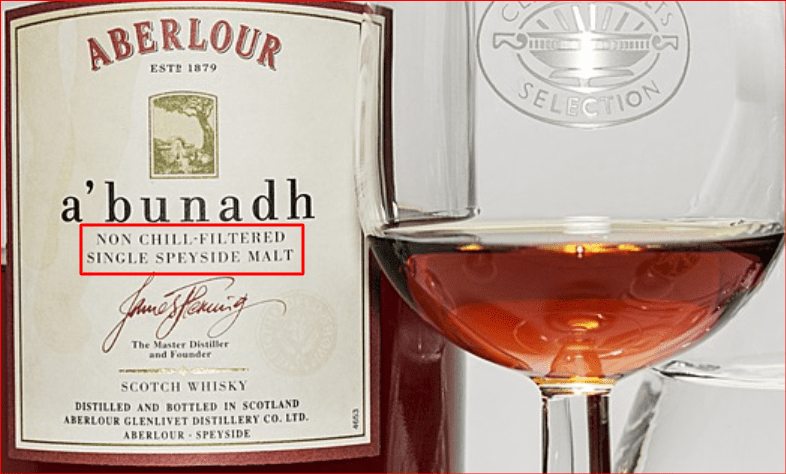
\includegraphics[totalheight=6cm]{figures/onchillfilt.png}
 	 	\end{center}
 	 	\caption{Non chill filtered clearly advertised with pride on the label. Also, one of my favorite whiskies with a rich and lovely mouthfeel.}
 	 \end{figure}
 	 Finally, the cask maturation attributes were one-hot encoded. The chill-filter and cask-strength attributes were set to booleans.
 	 \subsection{Flavor descriptors: text normalization, tokenization, bag of words (BoW)}
 	 \paragraph{'Palate', 'nose', and 'finish' attributes:} 
 	 
 	 These are where all the flavor descriptors for Scotch reside. Let's take a look at an example from one whisky:
 	\\
 	\textbf{The GlenDronach 18 Year Old Allardice}
 	 \\
 	  \textbf{nose}: "Sherry notes so thick you need a knife to cut them! There's a hint of old rum in there too, with pineapple and brown sugar in tow." \\
 	  \textbf{palate}: "Christmas cake, rum again, chocolate-coated hazelnut, runny honey and a hint of Sauternes." \\ 
 	  \textbf{finish}: "Fresh blackcurrant, blueberry pancakes with a generous helping of maple syrup."
 	  \\
 	 
 	 The text for each of these attribute is informative but fairly short. Another point is that the three attributes (perhaps unsurprisingly) are related to each other. There is a lot of sweetness, dark sugars, fruit, etc. Given these points, I decided it didn't make sense to create three separate dictionaries/corpuses and instead joined the text from the three attributes in order to create a unified token set.
 	 \paragraph{} After combining the text, each document was passed through another Spacy pipeline. We passed the text into Spacy's lemmatizer and removed stop words (some custom words were added based on data exploration) and punctuation. We also removed verbs and adverbs as most relevant flavor descriptors are either nouns or adjectives. We then found relevant bigrams in the text. Taking a look at the text for the Glendronach 18 taste notes above, one can imagine that "brown sugar" or "maple syrup" occur a reasonable amount in the entire set of Scotch reviews. It makes sense to find these pairs and tokenize them not as independent words but as bigrams. We trained a Gensim Phrase model that uses the conditional probability of one word preceding another to do this for us. Let's see what happens after this process: \\
 	 \textbf{The GlenDronach 18 Year Old Allardice (tokenized)}: 'christmas\_cake', 'rum', 'chocolate', 'hazelnut', 'runny\_honey', 'sauternes', 'sherry', 'thick', 'knife', 'old', 'rum', 'pineapple', 'brown\_sugar', 'tow', 'fresh', 'blackcurrant', 'blueberry', 'pancake', 'generous', 'helping', 'maple\_syrup'.
 	 \paragraph{} We then ran a manual stemmer on the remaining unigrams. The reason we needed to do this was that Spacy's lemmatizer doesn't connect words like "malty", "malt" and "maltiness" together. The same goes for words with modified endings like "-ied", "-ness" (e.g., sherry/sherried, rich/richness). This stemming/replacement was implemented by regex substitution. A list of all the replacement rules we implemented are in the Data Wrangling notebook. 
 	 
 	 The resultant tokenized documents were then used to define a Gensim dictionary. This is essentially a hash table for looking up whether a given word exists in the corpus. The process resulted in approximately 4100 unique tokens. Gensim's dictionary object supports filtering out tokens that appear too frequently or too infrequently. These tokens are not useful in building models to understand relationships between the tokens or between documents. We thus filtered out tokens that appeared in more than half the documents and tokens that appeared in less than 0.5\% of the documents. After this filtering, the number of unique tokens in the dictionary dropped to 477. We then used this reduced dictionary to create a Gensim bag-of-words corpus (essentially a sparse document/token-frequency matrix).
 	 \section{Exploratory Data Analysis}
 	 \subsection{Visualing the space of flavor descriptors}
 	\paragraph{} We want to visualize the space of descriptors. First, it's just a good idea to see whether our tokenization process produced a dictionary that makes sense (vs. having a lot of irrelevant tokens). We also want to get a picture of which descriptors are frequent across all the Scotch tasting notes. A wordcloud does a good job with this:
	 \begin{figure}[H]
	 	\begin{center}
	 		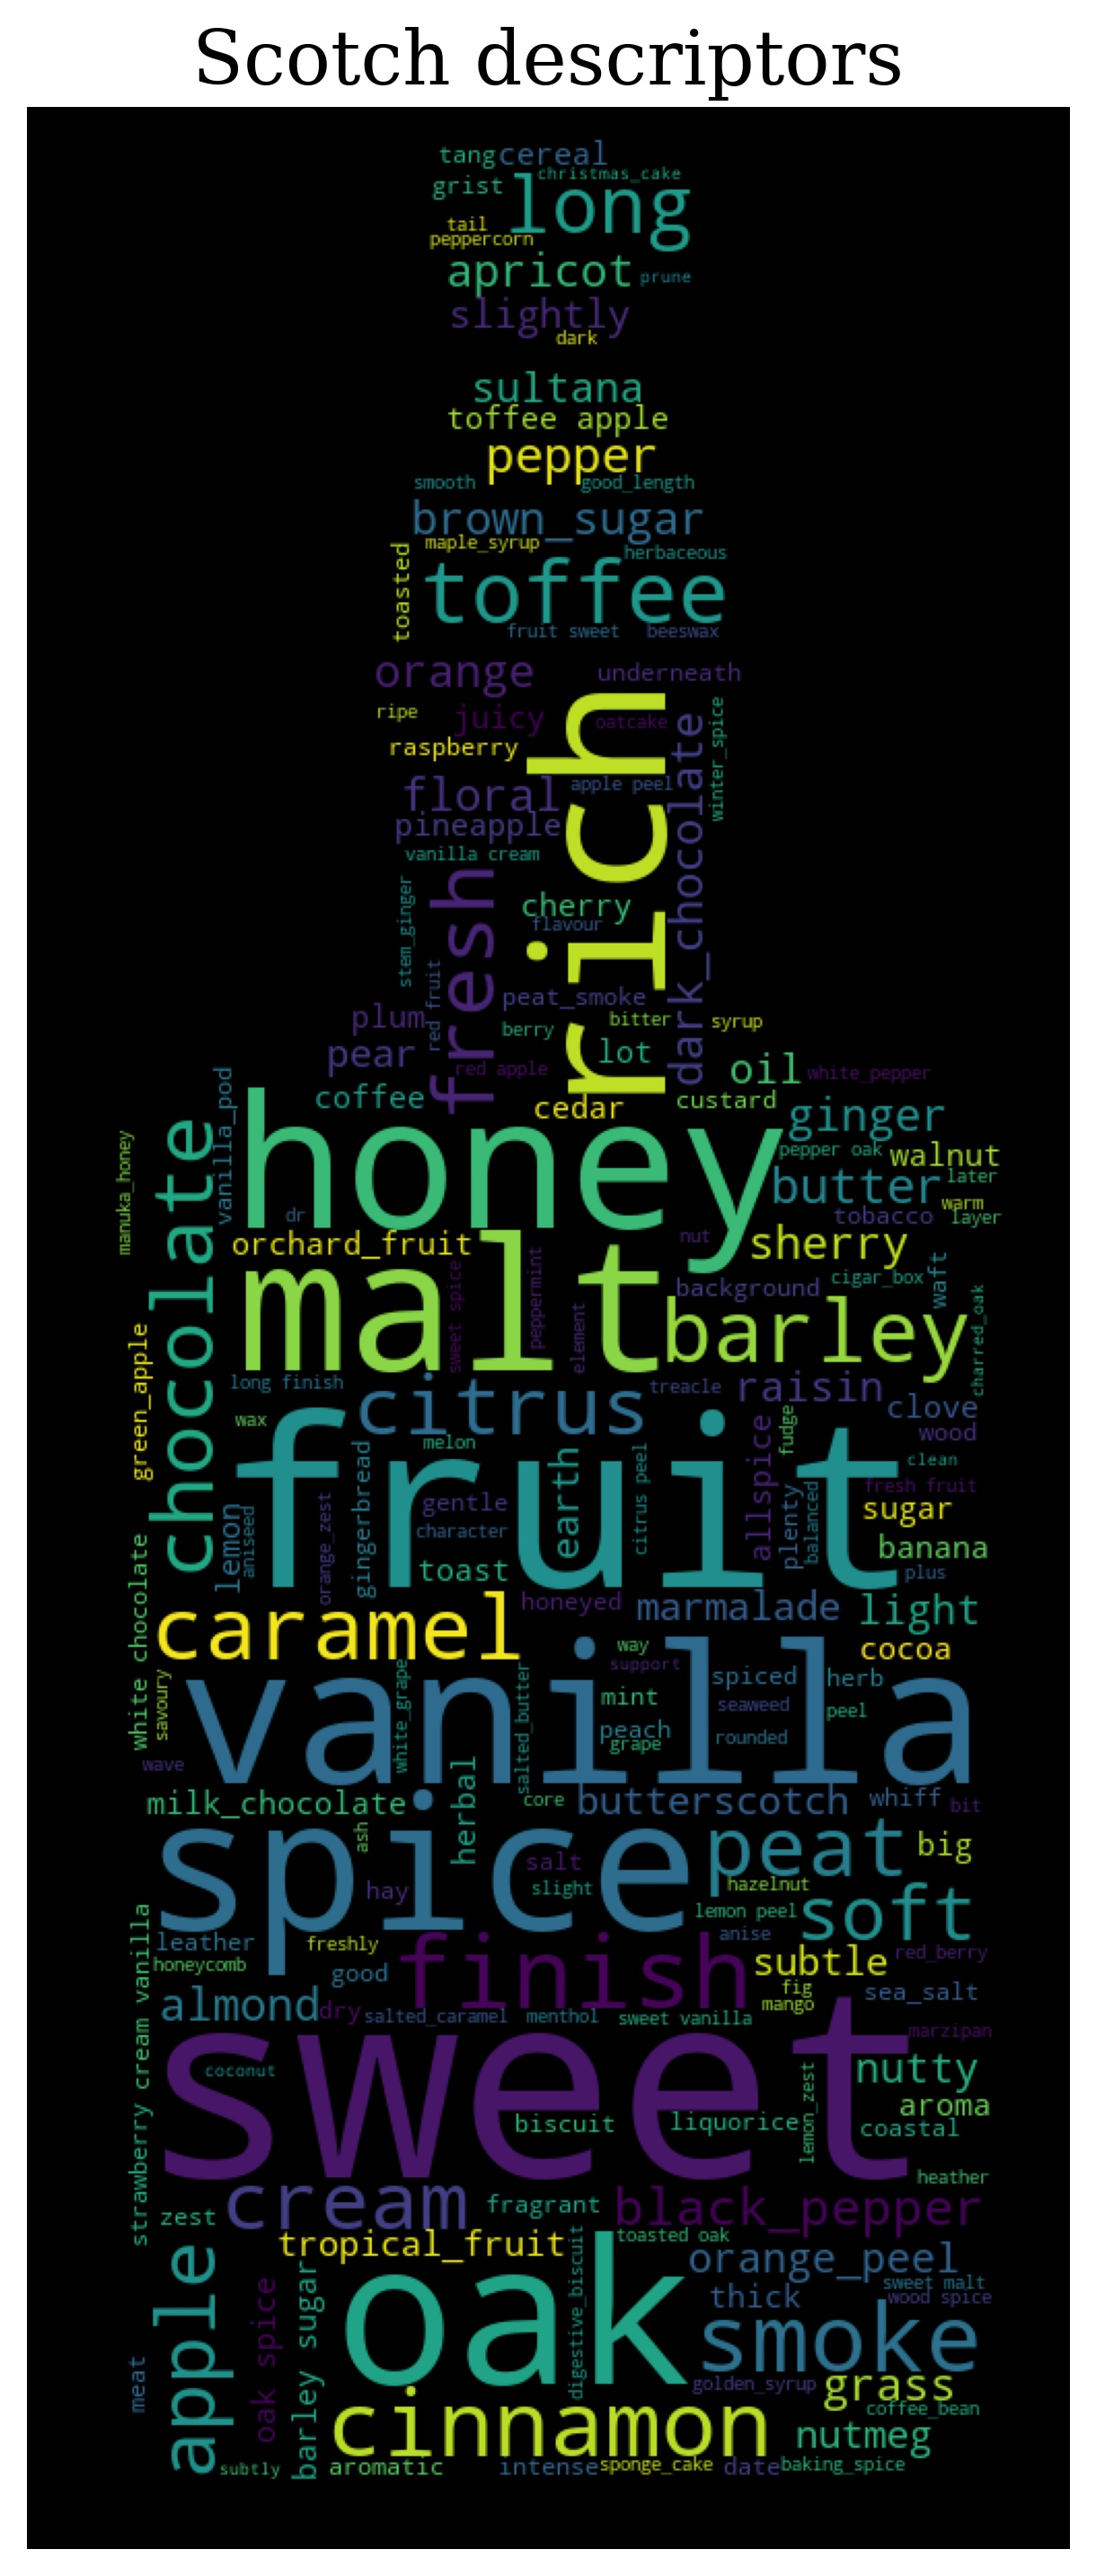
\includegraphics[totalheight=12cm]{../images/EDA/wc_token_unified.jpg}
	 	\end{center}
	 	\caption{Wordcloud of Scotch reviews restricted to the 477 tokens of the reduced gensim dictionary.}
	 \end{figure}
	 \paragraph{} An inspection of these words show us that our tokenization is working pretty well...most of these are flavor descriptors and there is (at least in the most prevalent tokens) no sign of two different forms for the same word. The most frequent  descriptors throughout the tasting notes are 'sweet', 'fruit', 'spice', 'vanilla', 'oak', 'rich', 'honey', 'smoke'. The question is whether these descriptors are common across all the reviews or whether they belong to a subclass that is very large. We need to dig deeper than a wordcloud to figure this out.
	 \paragraph{} One thing that can be done is to visualize token frequencies conditioned on some variable that we think might separate out different groups of descriptors. There are different Scotch producing regions in Scotland and it's often said that whiskies from the different regions tend to have different character. So let's do a term frequency breakdown by region:
	 
	 	 \begin{figure}[H]
	 	\begin{center}
	 		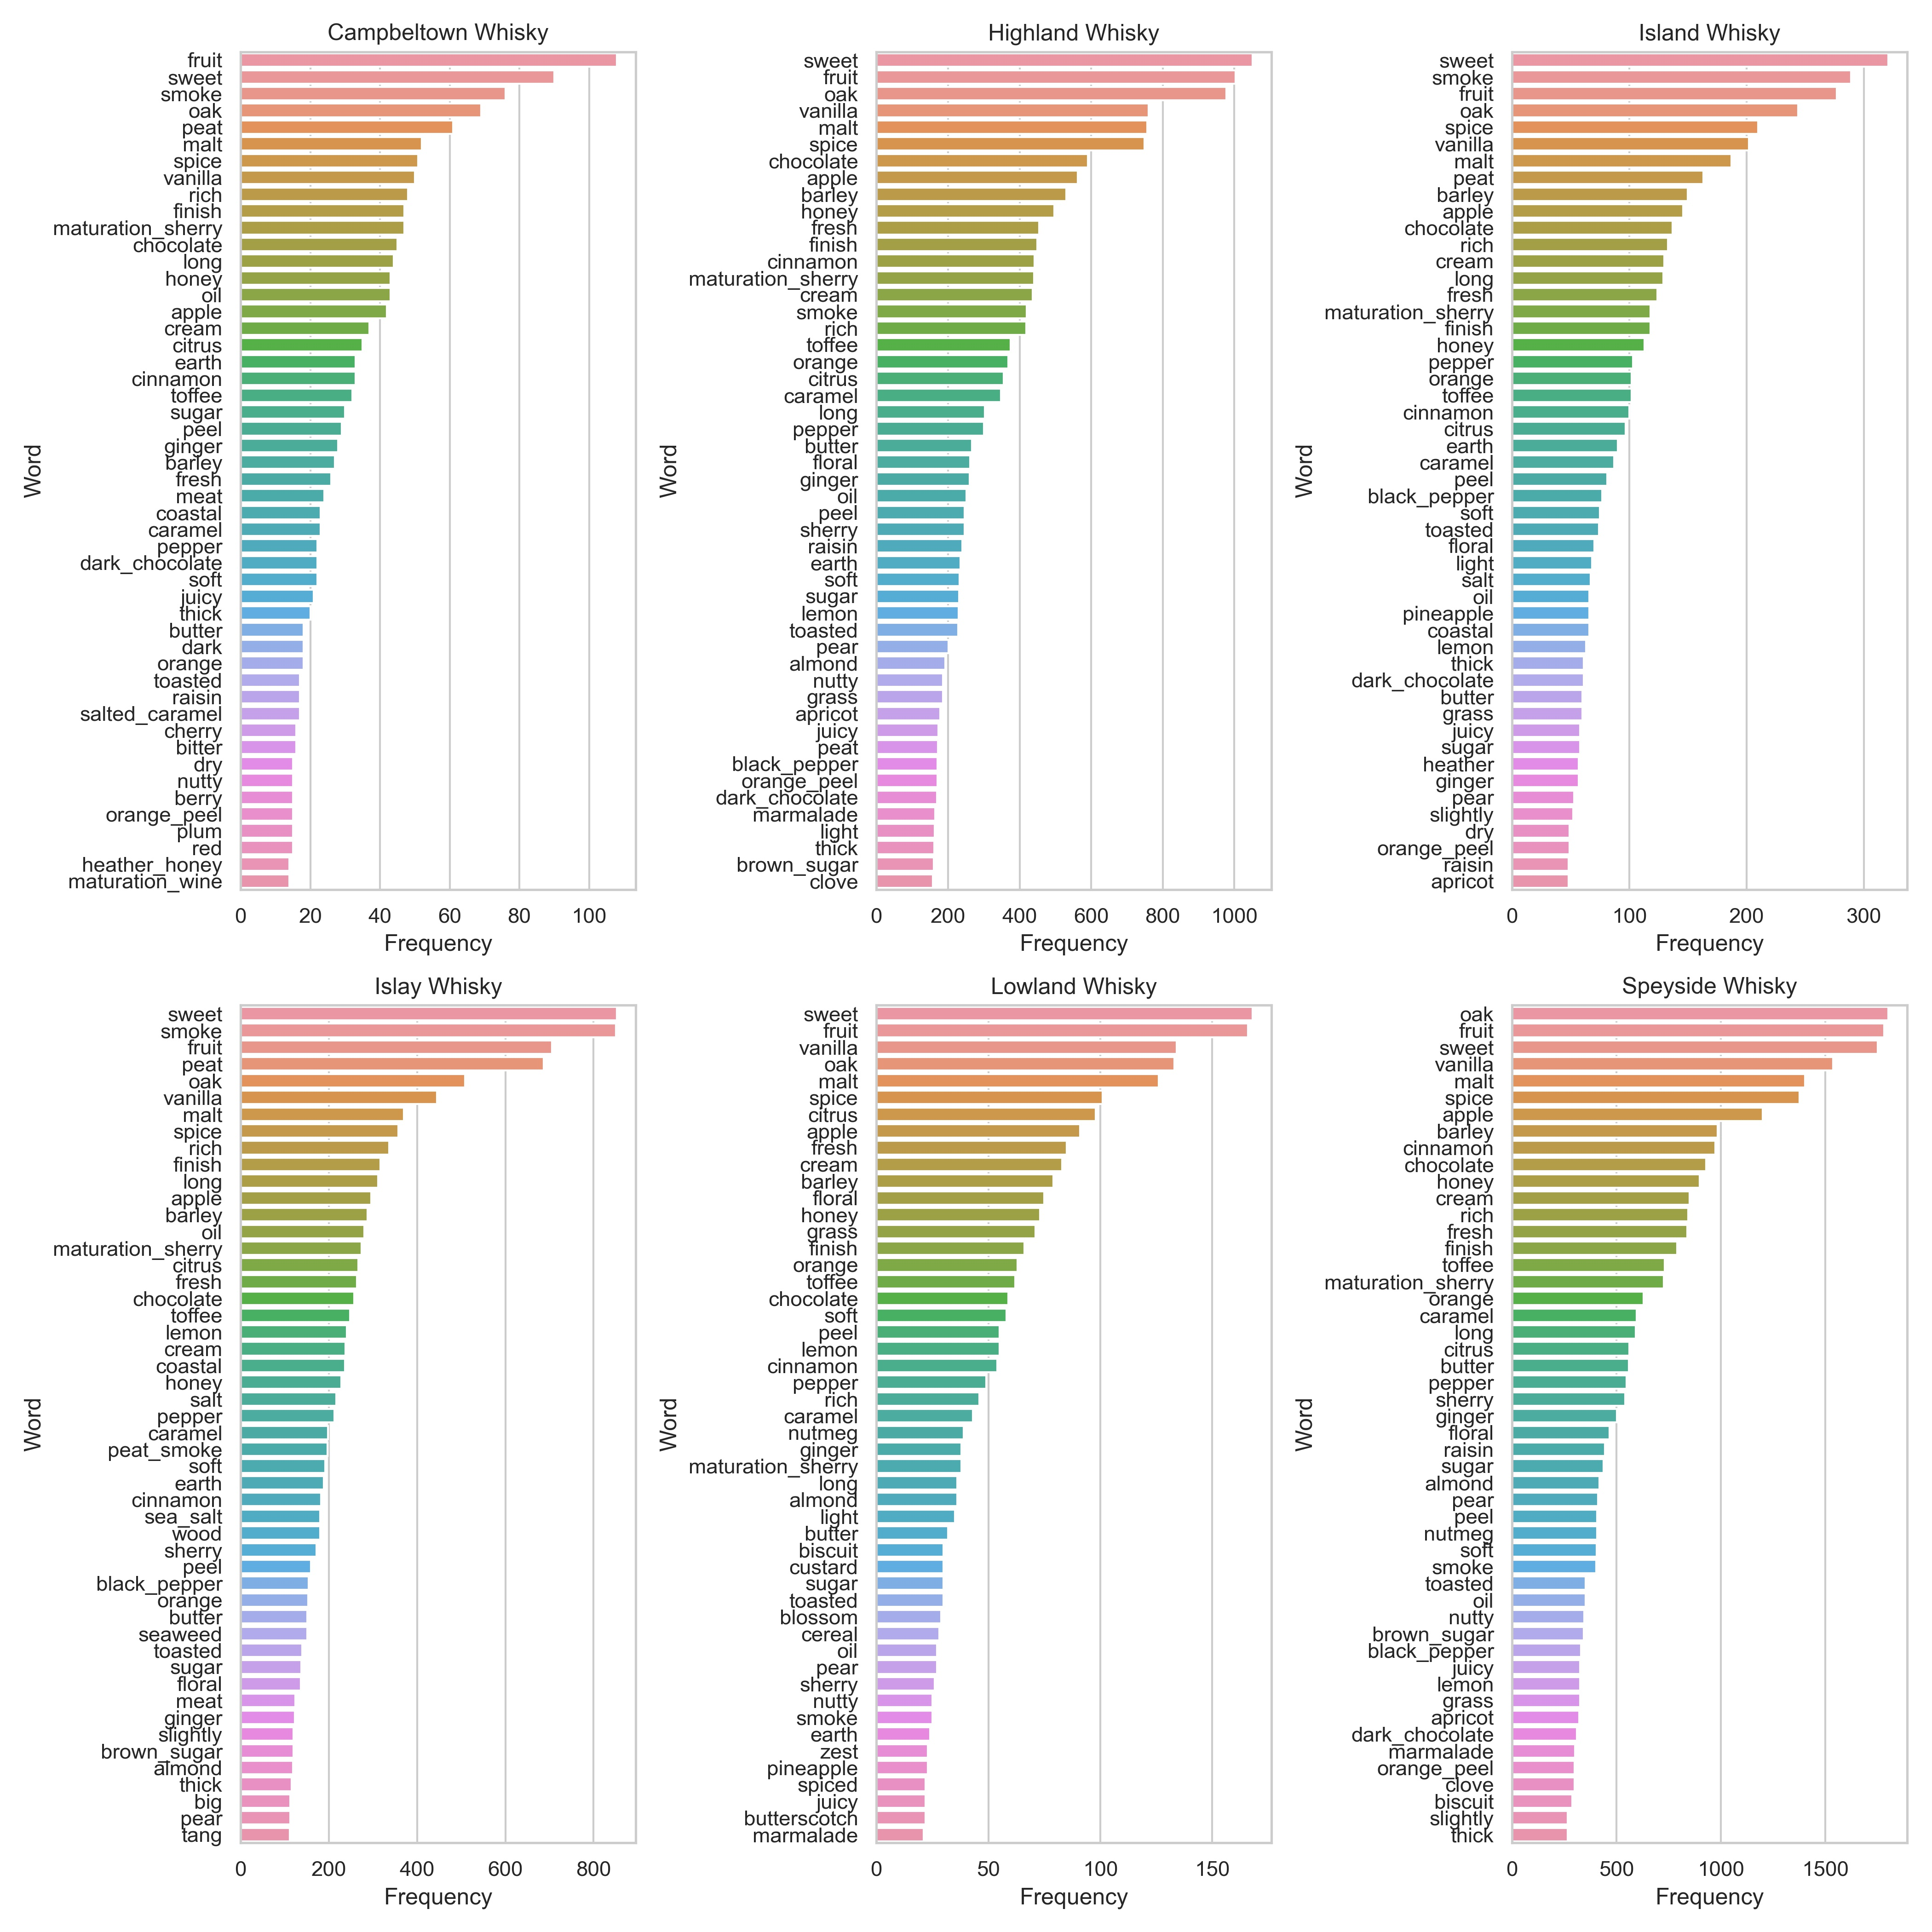
\includegraphics[totalheight=13cm]{../images/EDA/topwordsbyregion.jpg}
	 	\end{center}
	 	\caption{Thirty most frequent Scotch descriptors broken down by region.}
	 \end{figure}
	'Fruit', 'sweet', 'vanilla', 'malt', 'spice', and 'oak' seem to be very high up on the count frequency list for ALL the regions. These are definitely common descriptors of Scotch. One thing to note is that 'fruit', 'sweet', and 'spice' are also pretty generic words in the flavor universe. "Malt" and "oak" being a common descriptor for Scotch is not surprising either (given Scotch is made from malted barley and typically aged in oak barrels). There do, however, seem to be some regional differences. 'Smoke' appears high up on the list for Islay, Island, and Campbelltown regions. It's a little lower but still in the top 30 for Highland. 'Smoke' doesnt appear for the Lowland and Speyside regions. Islay, Island, and Campbelltown whiskies have descriptors that are not prevalent in the other regions: coastal, salt, sea salt, peat smoke, meat, seaweed, etc.  
	\paragraph{} Clearly, there is something to the notion that there are regional characters to the whisky. It also makes sense that the terms that are extremely frequent and common across all the categories are either terms that are pretty generic or would make sense given the general Scotch making process. The tricky part comes when we realize that there are descriptors a little farther down the list that are also frequent in every other region: raisin, black pepper, ginger, nutty, lemon, orange, earth, chocolate, etc. These are less generic terms. But do they belong to every whisky in a given region? Likely not. There are some whiskies with light citrus character and saltiness. Others in the same region are bittersweet and savoury/meaty notes. Which of the many flavor descriptors correspond to these taste groups? We thus need to find structure within the descriptors themselves. We would also want to situate each Scotch within the space of these descriptor groupings. We then might be able to say whether a Scotch has a predominantly salt and smoky character or whether it has a light/floral character.
	\subsection{Correspondence Analysis} \paragraph{} There are a variety of embedding techniques that can do this. For visualization, we'd like the ability to embed and transform/project into a low-dimensional subspace. We chose to use a technique known as Correspondence Analysis. The technique essentially calculates the expected value of every element of the document/term-frequency matrix by first computing the weight of a given term in the entire corpus and then multiplying it by the average term frequency across all terms for a given document. The resultant matrix is essentially the document/term frequency matrix assuming there's no correlation between particular documents and particular sets of terms. Subtracting this matrix from the original document/term-frequency 
	yields a \textbf{residual}.
	\paragraph{}  Document/term-frequency elements with high positive residuals suggest that a document is associated strongly with a given term. This also means that terms with similar residuals across a wide variety of documents can be said to be related to each other. Calculating the embedding is essentially a matter of taking the SVD of the residual matrix, getting the document and term coordinate system from this, keeping the coordinates with the largest singular values, and scaling the document/term coordinates appopriately to not distort dot-products, etc. The result of the embedding for the descriptors can be seen below: 
	
		 	 \begin{figure}[H]
		\begin{center}
			\includegraphics[totalheight=14cm]{../images/EDA/CA_word_embed.jpg}
		\end{center}
		\caption{2D embedding of Scotch descriptors using Correspondence Analysis.}
	\end{figure}
\paragraph{} There is actually some noticeable structure here (despite the big dense blob of descriptors in the center). The region close to X=0 and $Y< -0.5$ have pretty similar characteristics: 'christmas', 'raisin', 'christmas\_cake', 'fruitcake', 'liqueur', 'pudding', sultanas', 'sticky\_toffee', 'stewed', 'fig', 'rum', 'molasses', 'treacle', 'marzipan', 'date', 'nutmeg', etc. These are all very thick, sweet, deep sugary, sweet-spice and holiday-like flavors.

A little further up in Y closer to 0 and for $X < 0$ near the Y-axis we get 'jam', 'blackberry', 'raspberry', 'peach', 'apricot', 'strawberry'. It's hard to see but 'red\_currant, black\_currant, golden\_plum and red\_berry are in this region too. These descriptors are similar: a combination of fruity sweetness and tart flavors. As we go over to large $X > 0$ and $Y<0$ we have cocoa, mixed peel, aniseed, star anise, manuka honey, pipe tobacco, espresso, bittersweet. These are all tastes balanced between bitter and sweet or having notes of both. As we go higher in Y from here, we start to get (roughly speaking) more astringent and sour notes: rhubarb, tannin, acacia, wine,...and going further up in Y and closer to X = 0: 'citrus', grapefruit', 'dry', 'grass', 'crisp', 'lemon\_'zest', 'fennel'...etc. At even higher $Y > 1$, we also see a distinct set of flavors that are grouped together. These are salty, smoky, savory notes: "salt", "coastal", "seaweed", "iodine", "peat", "peat\_smoke", "meat", "ham", "charred", "bbq", "bonfire", etc. 
\paragraph{}
We've identified groupings of words that have meaning in terms of distinct flavor types in the context of Scotch whisky. The descriptors don't separate into distinct clusters. Rather we can describe this as more of a continuum. This makes sense, given the way Correspondence Analysis works and that Scotches are complex and a single Scotch may contain many (seemingly opposite) types of flavor. Scotches embedded in the same space also exhibit no clustering. But when we condition on region, we do see some structure emerge. The 2D hexplots show that Speysides and Lowlands do not have peat/salty/meaty notes. They are dominated by fruit notes, chocolate, etc. Island and Islay whiskies have significant density in the smoky, fiery, salty region. This corroborates what we saw in the most frequent token lists by region.
		 	 \begin{figure}[H]
	\begin{center}
		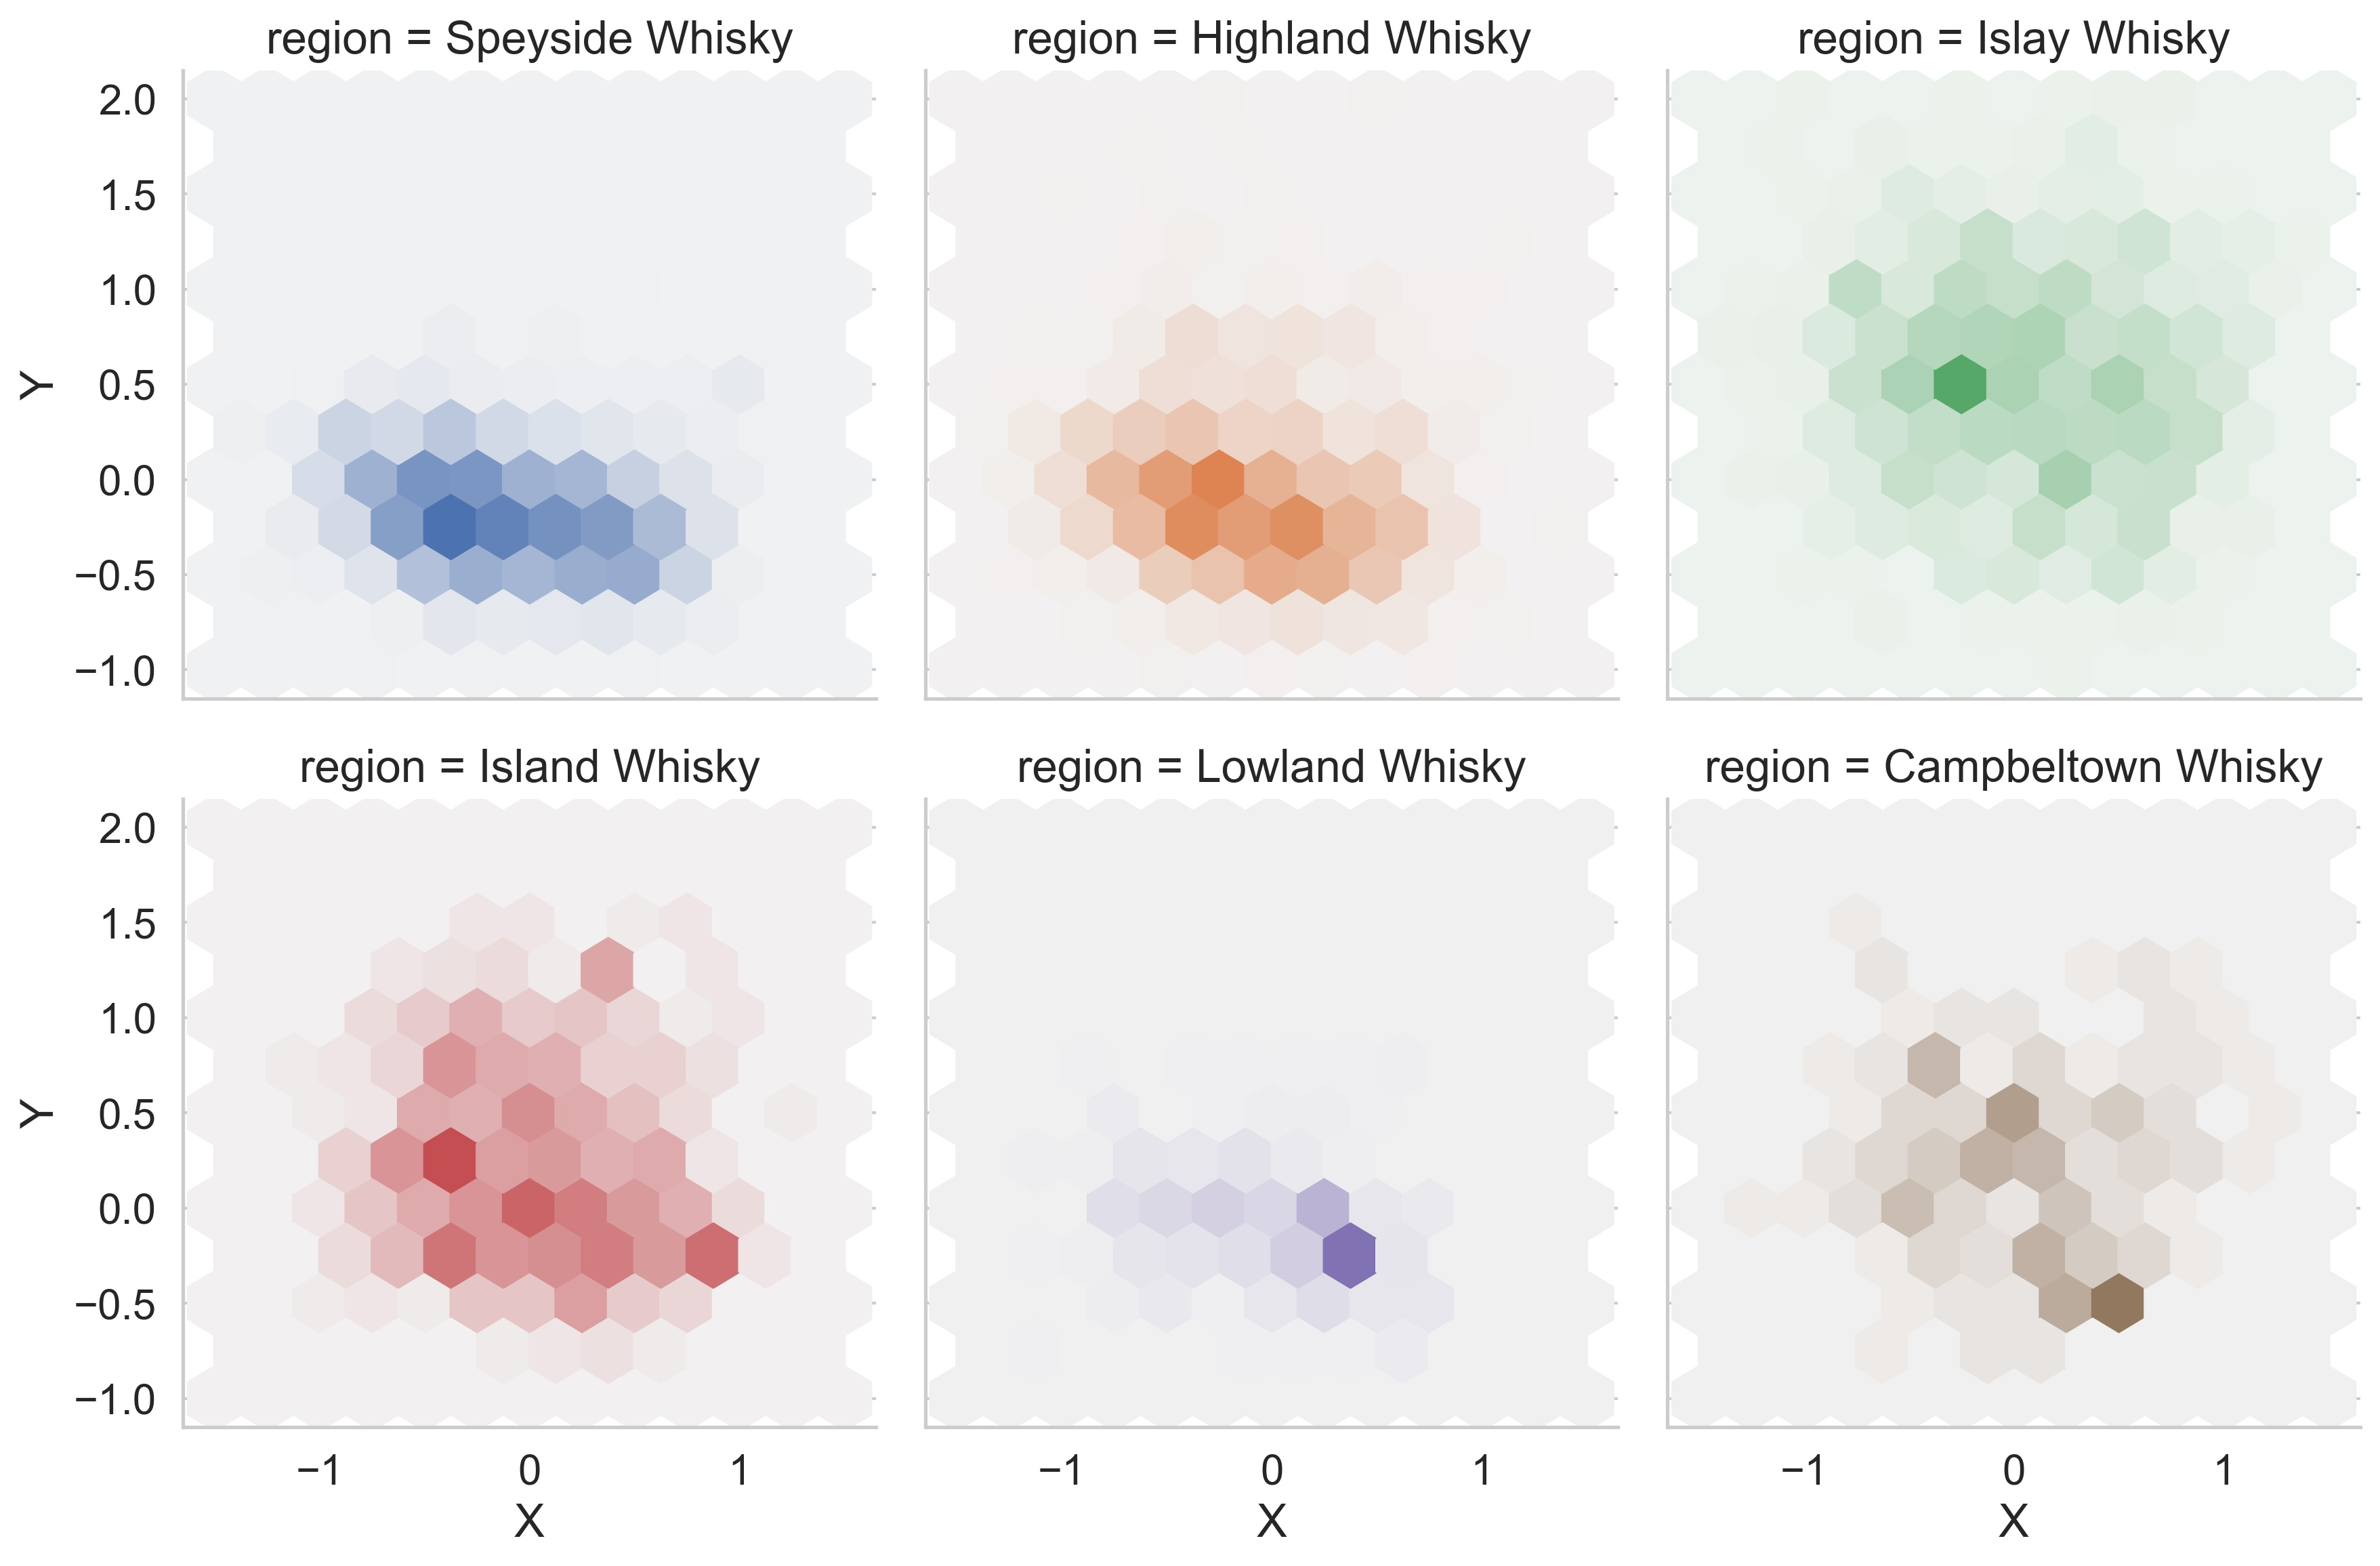
\includegraphics[totalheight=8cm]{../images/EDA/CA_scotch_hexdistbyregion}
	\end{center}
	\caption{Hexbin distributions of Scotches in the CA embedding space.}
\end{figure}
However, there is non-negligible density of scotches in the sweet sector for all of the regions -- even for Islay and Island scotches. This is more to the point that likely many salty, peaty, meaty, also have notes of toffee, caramel, etc. The problem is that this technique will locate the Scotch in a point that is in either of these sectors but cannot put them in both. The CA method of embedding thus may be good for visualizing the associations between tokens, but we want a way of decomposing the Scotches themselves into respective flavor components.
\section{Topic Modeling}
\paragraph{}We want to do topic modeling. We have a corpus of Scotch tasting notes and we are hypothesizing that this entire body can be described in terms of only a few "topics" -- or in this context flavor/scent types. Based on CA visualization, this hypothesis is reasonable. We do not expect that the words in each topic are completely disjoint. Judging by the dense cloud from the 2D CA visualization, there are words that might occur frequently between two types of flavors. An example would be "fruity." "Fruity" could go with "lemon", "zest", "grapefruit", "orange" or it could go with "mango","banana", "dates", "figs". Clearly, these flavor profiles are different but "fruity" applies to both lists. Thus one might expect that many words are context specific and can go into several topics but mean different things in each.
\paragraph{} Latent Dirichlet Allocation (LDA) is particularly apt for this problem. The algorithm assumes a two-level generative process for the descriptors in each tasting note. At the first level, it's assumed that a set of $K$ latent topics generates the descriptors in each tasting note (i.e. document). The topics are composed with varying weights from the words in the corpus. Both the probability of a document having a specific distribution of topics and a topic having a specific weighting of words in the corpus both naturally follow a multinomial distribution. However, the probabilities governing the observation of topic k in document i or whether word j is contained in topic k are unknown. These are the parameters of the multinomial distribution and are taken to be Dirichlet distributed . Learning these, of course, is the inference problem at hand. 
\paragraph{} There are two main computational methods for solving this Bayesian inference problem: Gibbs sampling and a variational EM algorithm. We use Gensim's default LDA model which uses variational methods. Gensim's LDA model takes in the reduced dictionary, our documents set in the form of a gensim BoW corpus, and a few hyperparameters. We had gensim automatically choose hyperparameters for the topic Dirichlet priors (the vector $\vec{\alpha}$). We, however, did manually tune the topic number $K$ in a range from 2 to 20 topics. The goal is to create a model where the words in each topic clearly have coherence (belong together) and where the different topics are reasonably separate in meaning. LDA is rather interesting in that, tuned correctly, it can actually produce topics that are human interpretable. Gensim has a wrapper for LDA models, that can calculate topic coherence and output a coherence score averaged over all topics. Fixing initialization conditions, the mean coherence scores as a function of topic number can be seen below:

		 	 \begin{figure}[H]
	\begin{center}
		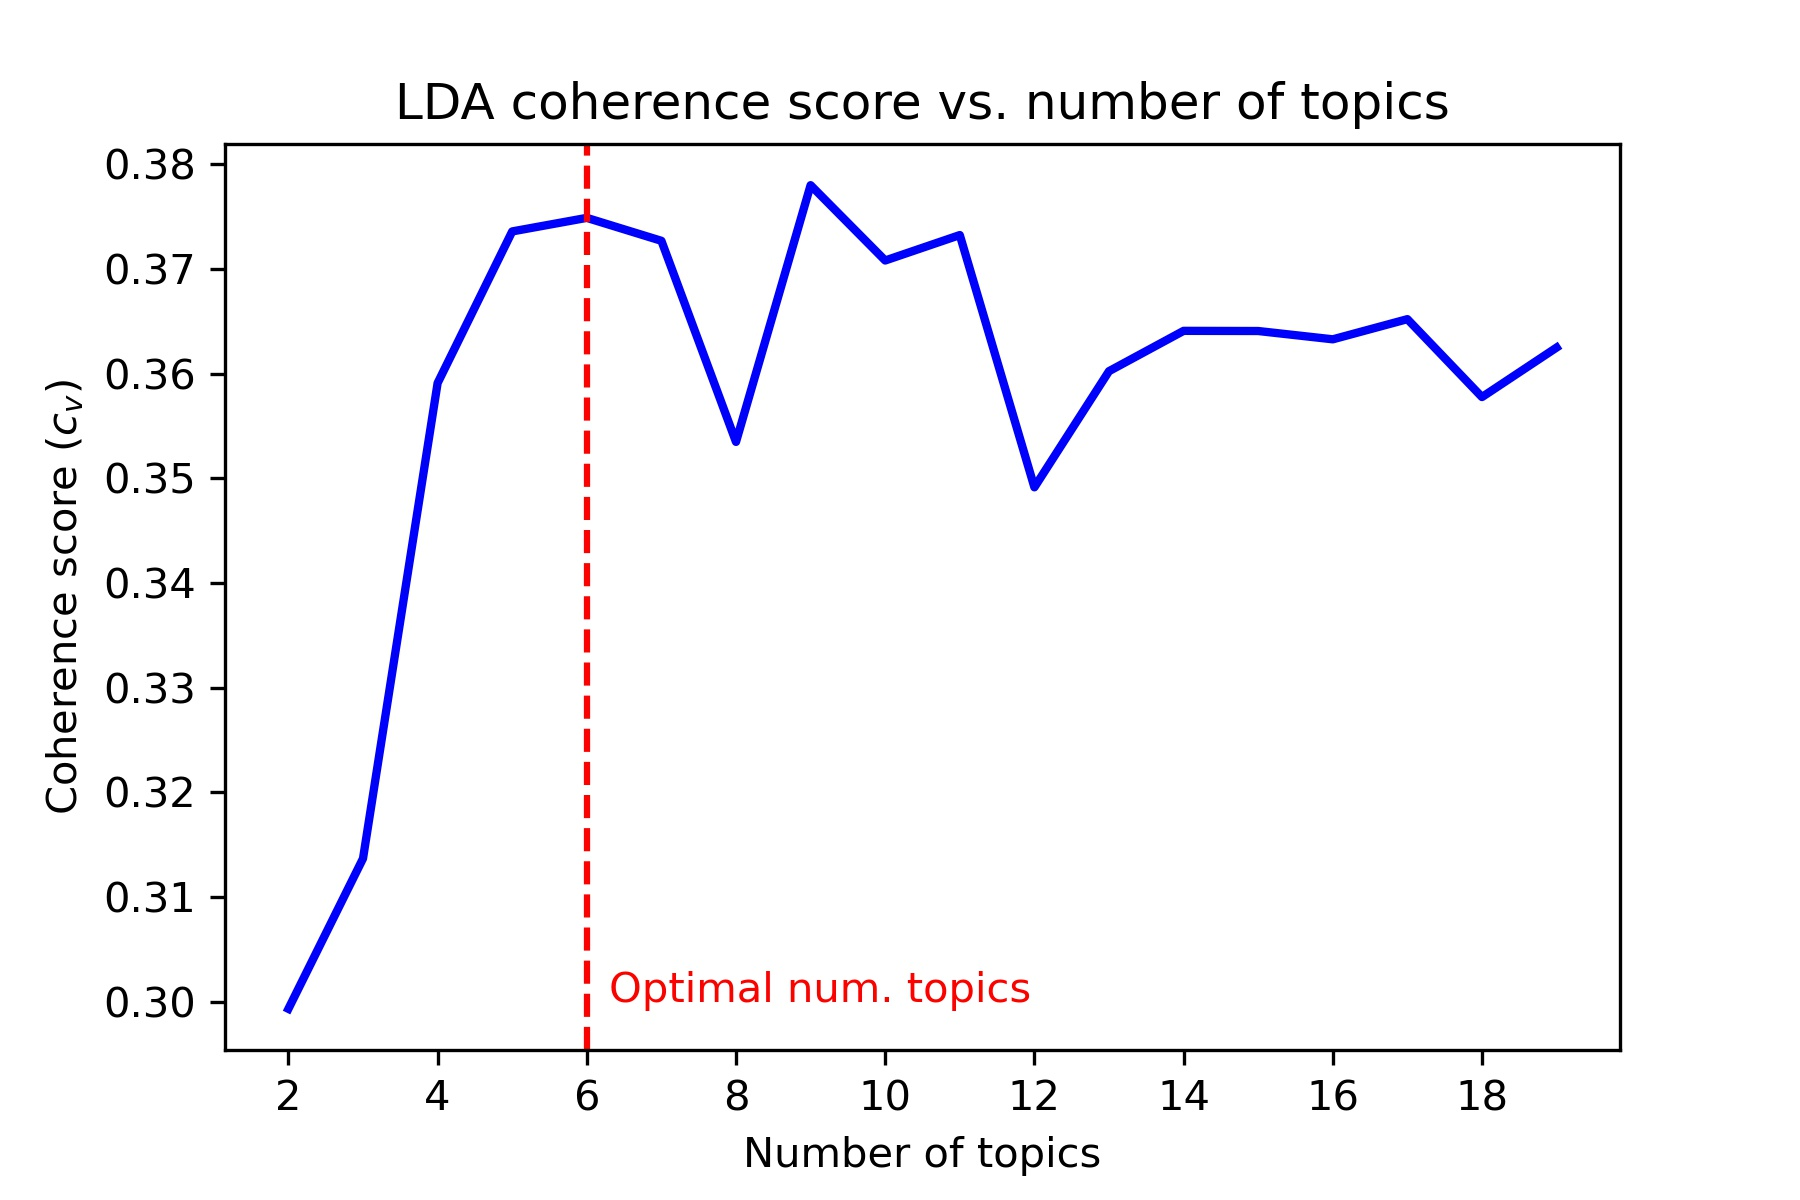
\includegraphics[totalheight=6cm]{../images/Modeling/LDA_coherence}
	\end{center}
	\caption{Coherence scores vs. number of topics in LDA model. We chose k = 6 as the optimal number of topics. }
\end{figure}

\paragraph{} The topic coherence shoots up and levels out at around k = 6 topics. We wanted to have as large a mean coherence as possible while keeping the model reasonably simple. So it made sense to choose k = 6 as the number of topics for our model.  A pyLDAvis visualization of the intertopic distance and topic size shows that the model could be good:

		 	 \begin{figure}[H]
	\begin{center}
		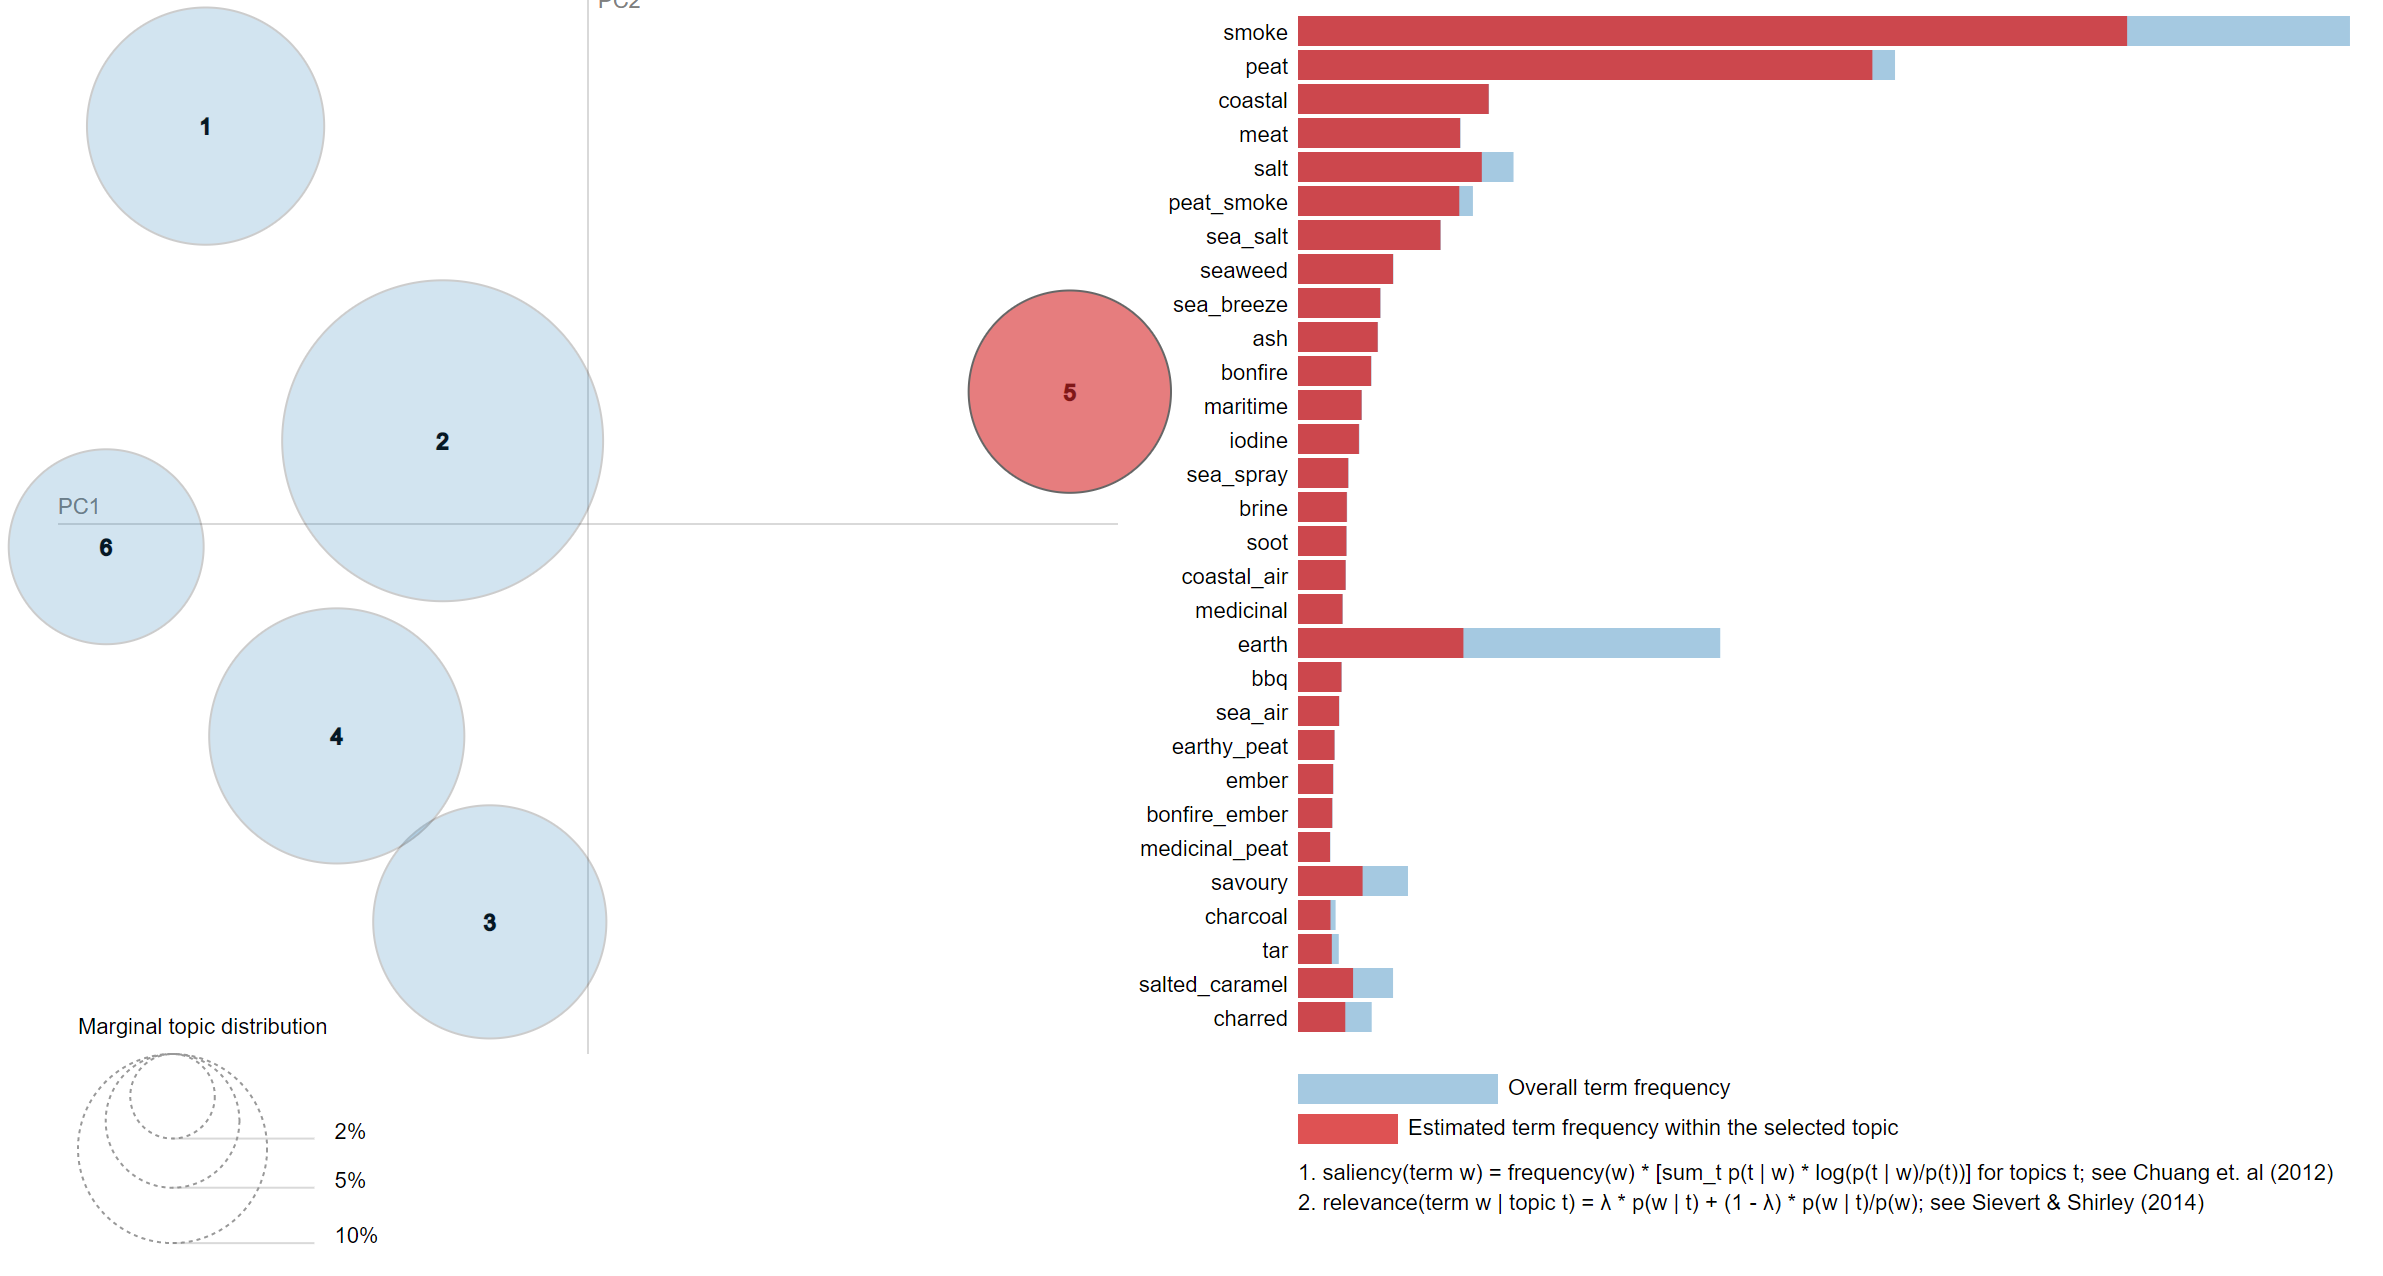
\includegraphics[totalheight=6cm]{../images/Modeling/PyLDAvis_topmodel}
	\end{center}
	\caption{Plot of the intertopic size/separation for our topic model as plotted by pyLDAvis.  }
\end{figure}
\paragraph{} The topic sizes are relatively well balanced and there is very little overlap between topics. A display of the characteristic tokens in topic 5 shows a rather encouraging: smoke, peat, coastal, meat, salt, etc. This topic clearly forms the smoky/savory notes in the flavor spectrum of Scotches. We present a breakdown of the rest of the topics below:
\begin{enumerate}
	\item  Sweet, rich, spiced christmas flavors with a mix of nuts, candied berries, aromatice spice, and dark chocolate. These are dark, sweet flavors.
	\item Citrus and floral with cream, malty notes.
	\item Herbal, tannin, citrus, wood. Drier notes.
	\item Wood, smoke, and pepper/heat. But also with richness.
	\item Smoke, peat, salt, meat.
	\item  Berries of various kinds, rhubarb, dark chocolate, jam, fruits, tartness but sweet. 
\end{enumerate}
\paragraph{} These groupings of descriptors definitely show some coherent taste/smell themes. These are also groupings that are useful in terms of characterizing Scotches. In fact, we identified some of these in Correspondence Analysis of the document/term-frequency matrix. The real power of LDA, however, is that now we can break down a tasting note into different taste-types. This allows us to categorize different aspects of a multifaceted Scotch. Let's see this in action:

		 	 \begin{figure}[H]
	\begin{center}
		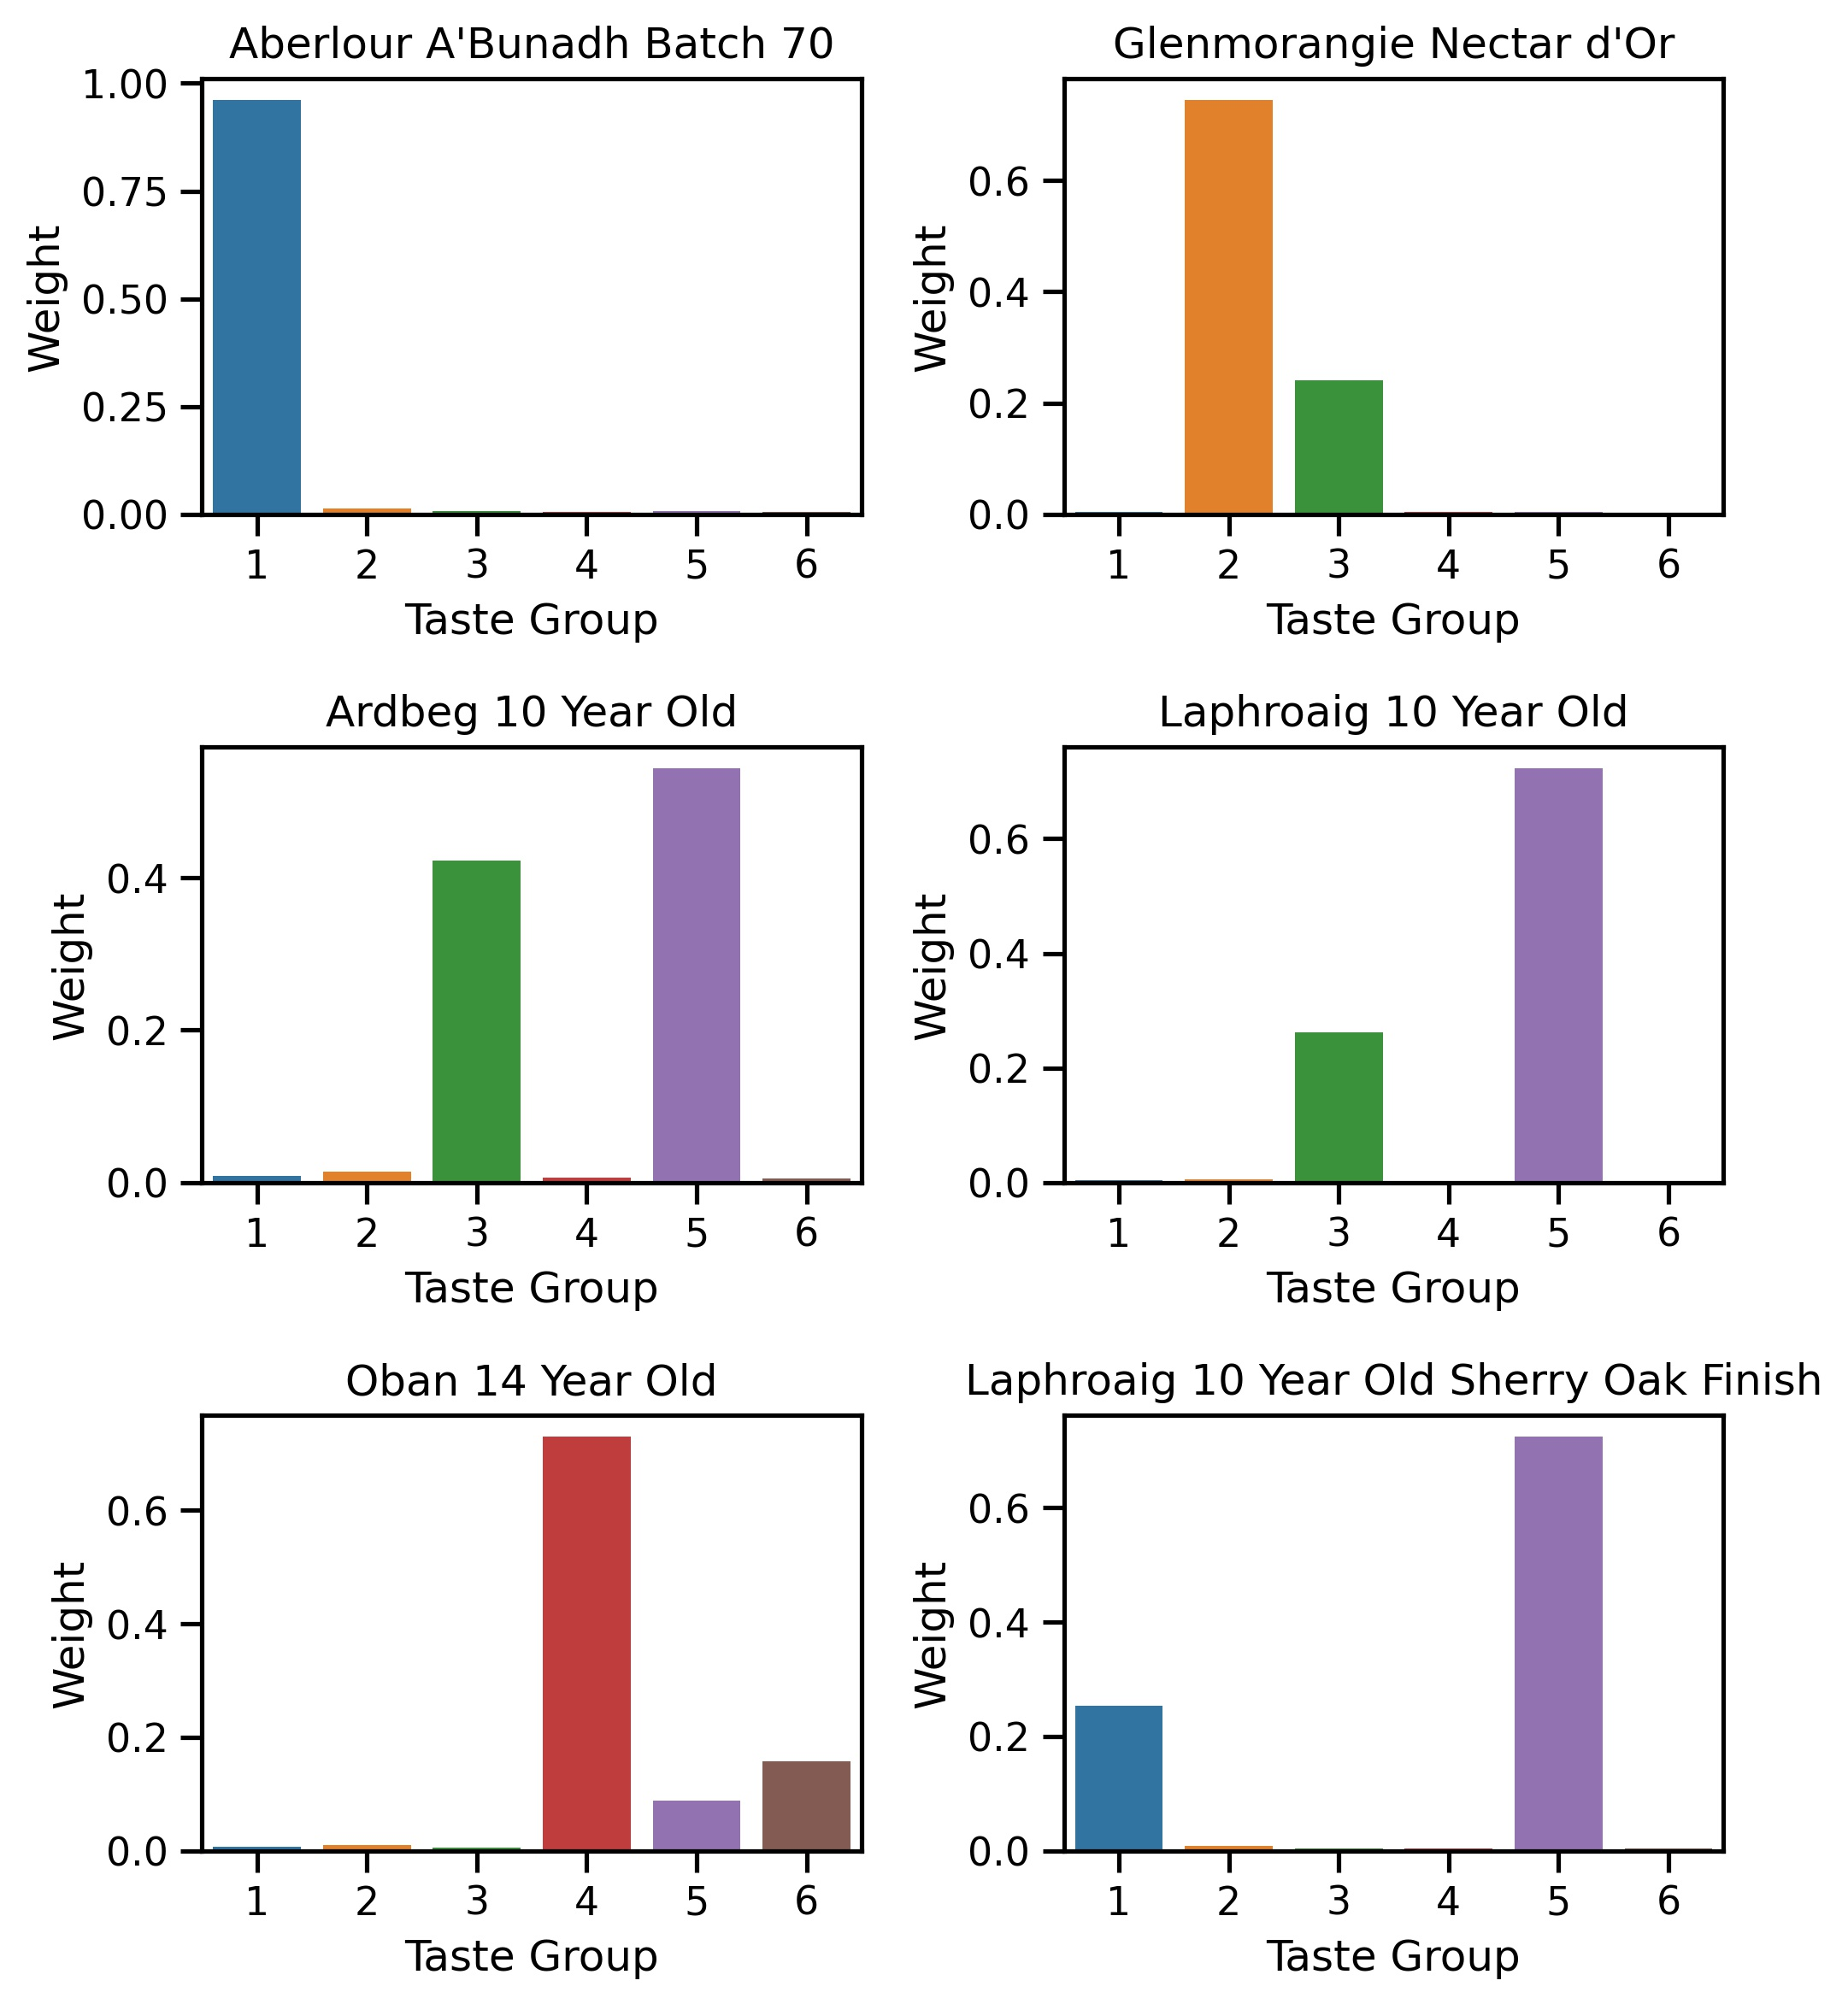
\includegraphics[totalheight=9cm]{../images/Modeling/scotch_topic_breakdown}
	\end{center}
	\caption{Scotch taste profile breakdown for some popular scotches.}
\end{figure}
\paragraph{} These are pretty good! Ardbeg 10 and Laphroaig 10 are both similar whiskies: Ardbeg 10 is a very peaty, fiery whisky with some dry citrus notes. Laphroaig is an extremely peaty, medicinal Scotch with herbal/wood notes. The taste profile breakdown gets this down. We tested whether the model would pick up appropriate changes in the flavor of a Scotch after a particular barrel finish. We take Laphroaig 10 with a sherry finish. According to the model, the finishing replaces the dry citrus accent with a dark fruit sweetness. This is consistent with what a sherry finish might do. Glenmorangie Nectar d'Or is a rich creamy whisky with orange citrus and grass notes. The model puts this whisky largely in taste group 2 which checks out. Arbelour A'bunadh is one of my favorite Scotches -- tastes like liquid Christmas. It's mainly been put into taste group 1. Nice. Finally, we check out Oban 14. It's a classic: a slightly salty, slightly smoky whisky with some tart fruit notes like apples or berries and wood spice. Again, our model is doing a decent job. In fact, it is doing well enough that we decided to build a content-based recommender with it.
\section{A Scotch Recommendation Engine}
We've represented the documents by vectors with the components representing different taste types. Given a particular Scotch, we want to find others that are similar in terms of topic breakdown. Scotches with topic vectors that have a small angle between them (i.e, a cosine similarity measure close to unity) are deemed similar.
\subsection{In-corpus Recommendation} For a given Scotch in the corpus, we get the cosine similarity of all the other Scotches in the corpus to the whisky in question. The ones with high cosine similarity imply good recommendations (i.e. whiskies with similar taste profiles to our input whisky). Let's evaluate this recommendation engine with a few whiskies as example:

\textbf{1. Laproaig 10 Year Old:} 
'seaweed', 'vanilla', 'ice\_cream', 'whiff', 'aid', 'box', 'tcp', 'plaster', 'etc', 'oak', 'big', 'way', 'fore', 'whisky', 'tongue', 'upsurge', 'spice', 'cardamom', 'black\_pepper', 'chilli', 'big', 'muscular', 'peat', 'spice', 'liquorice', 'big', 'dose', 'salt', 'whisky', 'slightly', 'sweet', 'recent', 'year', 'beauty', 'classic', 'iodine', 'plaster', 'cool\_wood', 'smoke', 'big', 'savoury', 'tarry', 'iodine'

\textbf{Some recommendations in the top 10}:\\
\textit{Torabhaig Allt Gleann - The Legacy Series}: 'bold', 'peat', 'coastal', 'tar', 'oil', 'texture', 'roasted', 'salted', 'nut', 'light', 'fruit\_salad', 'floral', 'waft', 'heather', 'fennel', 'metallic', 'medicinal', 'pepper', 'spice', 'wafts', 'wood', 'tobacco', 'crumbly', 'vanilla', 'shortbread', 'earthy\_peat', 'smoke', 'zing', 'lemon\_zest', 'salt', 'maritime', 'shellfish', 'sweet', 'fruit', 'apple', 'kiwi', 'vanilla', 'oak', 'big', 'hit', 'peat', 'smoke', 'sea\_breeze', 'harbourside', 'character' \\
\textit{Caol Ila 7 Year Old}: 'oak', 'smoke', 'peel', 'black\_pepper', 'sweet', 'rock\_pool', 'brine', 'sea', 'harbour', 'rope', 'lemon', 'beach', 'meat', 'soft', 'spice', 'wisp', 'iodine', 'smoke' 

\textbf{2. Aberlour A'bunadh}: 'gingerbread', 'orange\_zest', 'black\_pepper', 'thick', 'sherry', 'vanilla\_pod', 'christmas\_cake', 'cherry', 'bakewells', 'hefty', 'helping', 'cinnamon', 'cedar', 'cinnamon', 'raisin' \\
\textbf{Some recommendations in the top 10}:\\
\textit{Tamdhu 10 Year Old}:\\ 'soft', 'red', 'fruit', 'brown\_sugar', 'clove', 'chocolate', 'brazil\_nut', 'dry', 'orange\_peel', 'red\_wine', 'pecan', 'raspberry\_jam', 'crystallised\_ginger', 'cacao', 'juicy', 'blackcurrant' \\
\textit{Edradour 10 Year Old}: 'brown\_sugar', 'treacle', 'clove', 'cinnamon', 'load', 'raisin', 'walnut\_loaf', 'damson\_jam', 'richly', 'chocolate', 'rum', 'like', 'spice', 'chocolate', 'date'\\
\textbf{2. Glenlivet 12 Year Old}: 'butter', 'vanilla', 'rich', 'bright', 'fruit', 'apricot', 'pineapple', 'greengage', 'citrus\_blossom', 'toasted\_teacake', 'soft', 'crackle', 'oak', 'spice', 'malt', 'plus', 'red', 'apple', 'juicy'
\textbf{Some recommendations in the top 10}:\\
\textit{Glenmorangie X}: 'lot', 'vanilla', 'apricot', 'apple', 'flaked', 'almond', 'later', 'honeyed', 'malt', 'lemon', 'apple', 'plus', 'nutmeg', 'oak', 'warmth', 'honeyed', 'orchard\_fruit', 'theme', 'finish', 'pinch', 'peppercorn'\\
\textit{Tormore - Batch 2 (That Boutique-y Whisky Company)}: 'caramelised', 'orange\_peel', 'fresh', 'lime', 'grapefruit', 'support', 'apple', 'golden', 'barley', 'core', 'steamed', 'marmalade', 'pudding', 'flourless', 'orange', 'cake', 'crushed', 'almond', 'apple', 'peel', 'juicy', 'barley', 'crisp', 'fruit'
\paragraph{} These three whiskies have pretty different flavor profiles. The suggestions line up. Recommendations for Laphraig 10 are peaty, smoky, and salty with some citrus/oak, for Arberlour A'bunadh we get a lot of rich fruit, dark sweetness, and aromatic spices. Finally, for Glenlivet 12 we have a lot of bright fruit notes (citrus, apples), softness, and vanilla.
\subsection{Out-of-corpus recommendation}
We also built functionality for out-of-corpus recommendation -- that is, a recommender based off of user-inputed free text describing certain tastes and smells. The free text is sent through the text pre-processing pipeline, tokenized and then BoW vectorized based on the reduced dictionary. Then the BoW vector is sent into the topic model, broken into a topic vector, and rank similarities of Scotches within the corpus to the free text description. We show an example below where we want a recommendation for Scotches with some coastal and salty qualities, dry, but also light citrus sweetness. Here is the description of taste that we inputted: "\textit{light, citrus, lemon, grapefruit, dry, crisp, sea salt, salted caramel}".\\
A few top recommendations:\\
\textit{Caol Ila 10 Year Old 2009}: 'coastal', 'peat', 'whiff', 'citrus', 'vanilla', 'oil', 'barley', 'phenol', 'damp', 'oak', 'bright', 'zest', 'citrus', 'cask', 'finish' \\
\textit{Longrow Peated}: 'light', 'sweet', 'green', 'grape', 'rhubarb', 'great', 'contrast', 'big', 'blast', 'smoke', 'salt', 'leather', 'fore', 'maritime', 'combination', 'harbourmaster', 'jacket', 'salt', 'return', 'deeply', 'satisfying', 'ending' \\
\textit{Springbank 12 Year Old Cask Strength}: 'calm', 'eye', 'storm', 'heather', 'coriander', 'oregano', 'caramel', 'busy', 'harbour', 'industrial', 'maritime', 'aroma', 'water', 'grape', 'springbank', 'rhubarb', 'thick', 'heavy', 'smoke', 'industrial', 'massive', 'long'.
\paragraph{} These recommendation certainly capture the coexiatence of dry light/tart fruit and coastal/salt notes that we were looking for. Some of the scotches also have smoke in them (which we didn't specify). However, given the broad nature of the taste categories it's not going to be possible to make strict distinctions between peat/meat notes and salt/coastal ones (they are all prevalent in topic 5). Overall though, pretty good.
\section{Conclusion/Future Work}
\paragraph{} The dictionary that was developed provides a common language of taste/smell descriptors for Scotch whisky. We found that these descriptors could be divided into different meaningful sectors corresponding to general types of flavor profiles. Savory, smoky, and salty notes were on one side of the spectrum and sweet fruit, dark sugars, and aromatic spices were on the other. Scotches are complex and can exhibit many types of flavor groups at once. We wanted a model that could capture this. Our topic modeling of the Scotch tasting notes using Latent Dirichlet Allocation worked quite well in this respect. The topic breakdowns and the Scotch recommender all produced results that captured the general taste profiles of various classes of Scotch whisky.
\paragraph{} There is, of course, quite a bit of room for improvement. The topics, while being reasonably distinct, are not truly disjoint (e.g., there is definitely overlap between topic 1 and 6 or between 3 and 4). LDA topic components, however, are orthogonal and this can lead to the model failing to find similarities between two Scotches that actually have some similarity. We need a notion of generating topics and measuring contextual/descriptive overlap between these topics. There are also notions of strength and weakness of certain flavors (big peat, big smoke, hint of orange zest) that are not captured. Supplementing the topic model with a word2vec or BERT type word embedding might do the trick. That being said, it's quite impressive what a relatively simple model can do. The topic breakdowns and the cask maturation/age/ABV information be used to study the influence of maturation on tastes. I'm sure there are other types of higher level analytics that are possible.  More importantly though, it's good enough that I might just follow one of the recommendations for Aberlour A'bunadh and grab myself a bottle of Edradour 10 and warm myself with a whee dram of holiday spice and sherried fruit this evening.



\end{document}